\paragraph{}
In order to create and update a repository, a distinguished machine, the so-called \textit{\textbf{Release Manager Machine}}, is used. On such a release manager machine, a CernVM-FS repository is mounted in read/write mode by means of a union file system. The union file system overlays the CernVM-FS read-only mount point by a writable scratch area. The CernVM-FS server tool kit merges changes written to the scratch area into the CernVM-FS repository. Merging and publishing changes can be triggered at user-defined points in time; it is an atomic operation. As we can see, a CernVM-FS repository is similar to a versioning system repository.
\paragraph{}
Repositories are periodically updated: installation of a new release or a patch for an existing release. Each time only a small portion of the repository is modified. 
In order not to re-process an entire repository on every update, CVMFS has a read-write file system interface to a CernVM-FS repository where all changes are written into a distinct scratch area.
Union file systems combine several directories into one virtual file system that provides the view of merging these directories. These underlying directories are often called branches. Branches are ordered; in the case of operations on paths that exist in multiple branches, the branch selection is well-defined. By stacking a read-write branch on top of a read-only branch, union file systems provides a writable interface for the file system. 
\paragraph{}
Union file systems can be used to track changes on CernVM-FS repositories (Figure below). In this case, the read-only file system interface of CernVM-FS is used in conjunction with a writable scratch area for changes.

\begin{figure}[h]
\centering
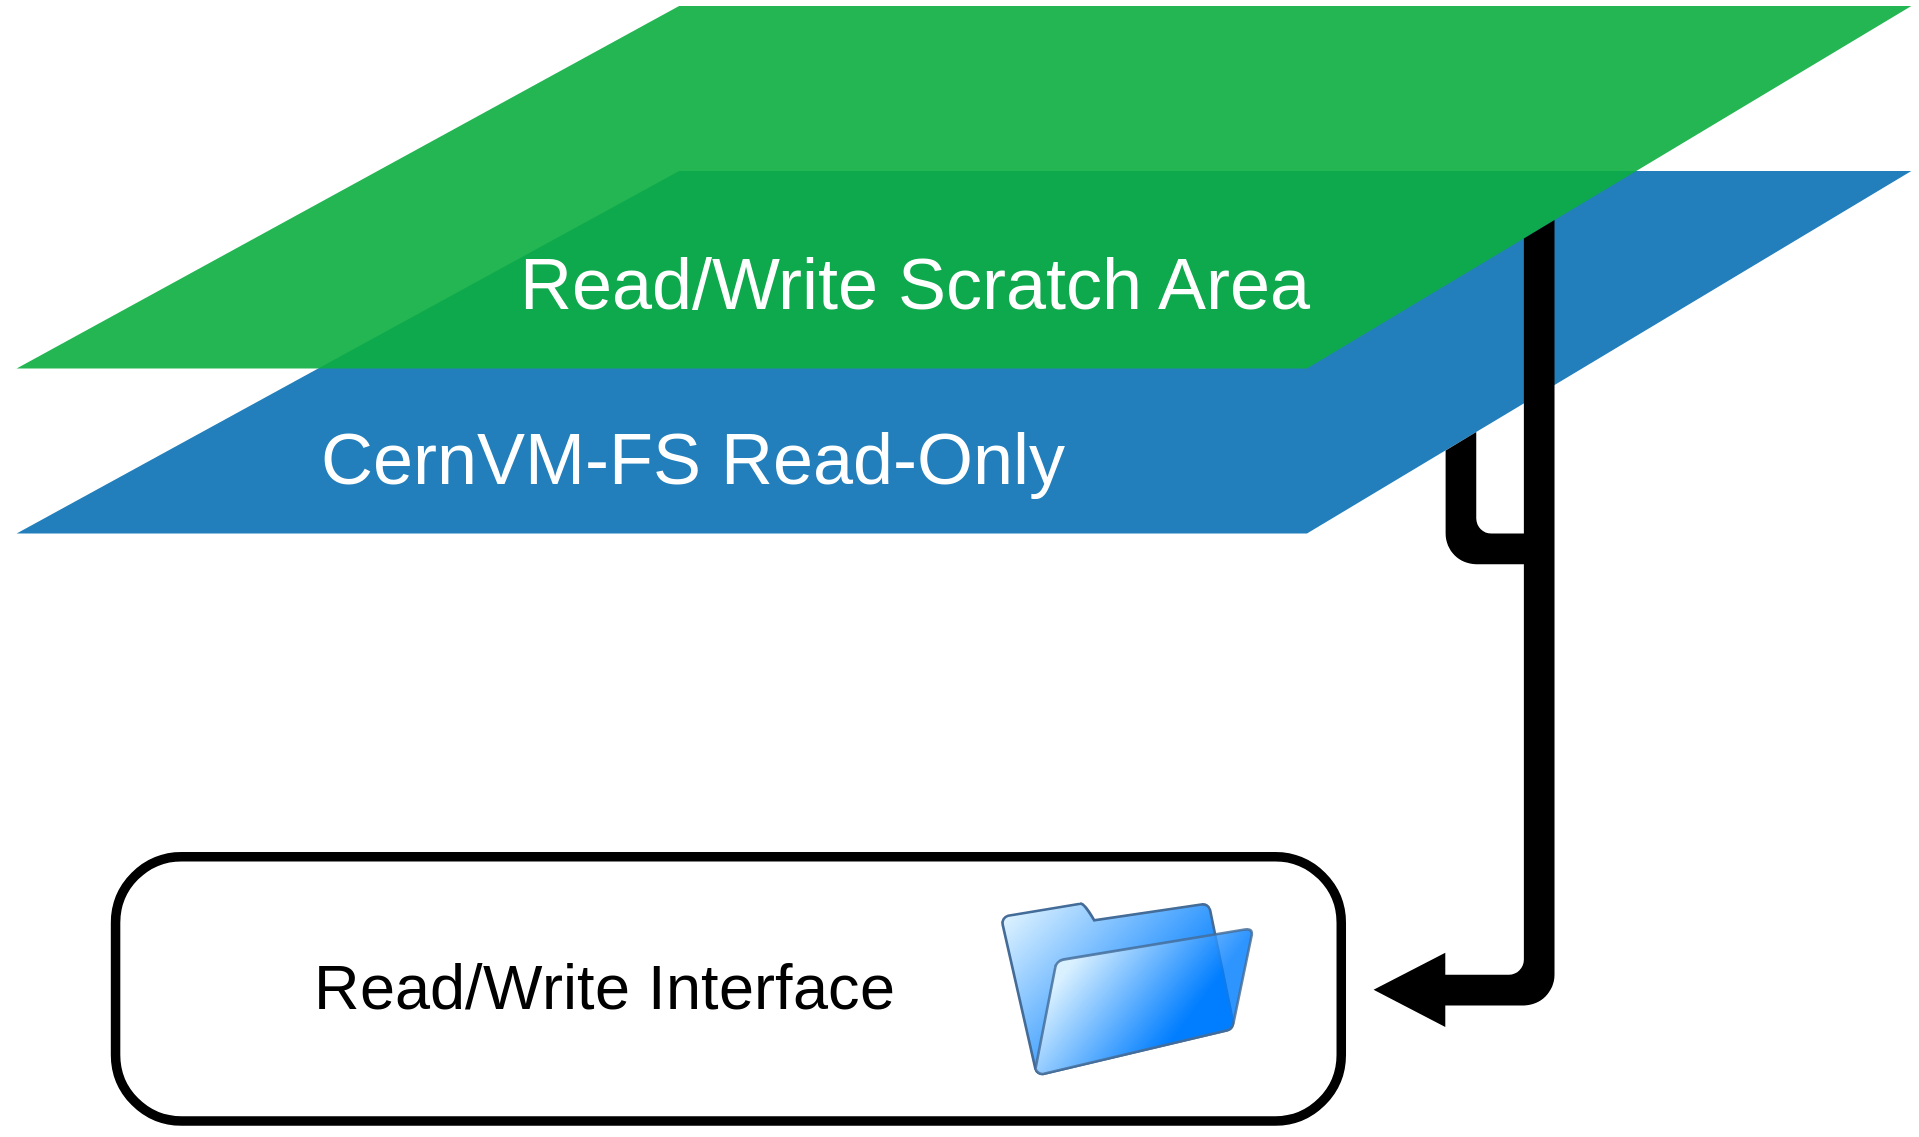
\includegraphics[scale=0.12]{figures/union}
\caption{\textit{A union file system combines a CernVM-FS read-only mount point and a writable scratch area. It provides the illusion of a writable CernVM-FS mount point, tracking changes on the scratch area.}}
\end{figure}

Change sets are published to CernVM-FS repositories through a transactional interface. Committing a transaction will increase the repository's revision number by 1 and make the new changes available to all repository clients.